\documentclass[10pt, landscape, french]{article}

\usepackage[utf8]{inputenc}
\usepackage[T1]{fontenc}

\usepackage[margin=0.8cm]{geometry}
\usepackage[document]{ragged2e}
\usepackage{minted}
\usepackage{multicol}
\setlength{\columnsep}{1cm}
\setlength{\columnseprule}{1pt}
\def\columnseprulecolor{\color{black}}
\usepackage[hyphens]{url}
\usepackage{graphicx}

\newcommand{\codeJSinline}[2] {
	#1 : \mintinline{javascript}{#2} \linebreak
  }

\newcommand{\codeHTMLinline}[2] {
	#1 : \mintinline{HTML}{#2}
  }
  
\newcommand{\codeCSSinline}[2] {
	#1 : \mintinline{CSS}{#2} \linebreak
  }

\newenvironment{codeJS}[1]{%
#1 :  %
\minted{javascript}%  % use \minted and \endminted instead of \begin{} an \end{} to solve errors...
}{%
\endminted%
}

\newenvironment{codeHTML}[1]{%
#1 :  %
\minted{HTML}%  % use \minted and \endminted instead of \begin{} an \end{} to solve errors...
}{%
\endminted%
}

\newenvironment{codeCSS}[1]{%
#1 :  %
\minted{CSS}%  % use \minted and \endminted instead of \begin{} an \end{} to solve errors...
}{%
\endminted%
}


\begin{document}
	
	\begin{center}
		\large{Feuille de triche HTML / CSS / Javascript}
	\end{center}

\begin{multicols}{3}

		\section{Javascript}

		\subsection{Syntaxe}
		% syntax stuff
		\begin{codeJS}{Les espaces ne sont pas pris en compte. Les tabulations permettent d'améliorer la lisibilité, mais ne sont pas importantes. Ces deux lignes sont équivalentes.}
var X =   1; 
var    X     = 1;
		\end{codeJS}
		\codeJSinline{Commentaires avec "//"}{// ce que je veux ici} 
		
		\subsection{Variables et types de base}
 		\codeJSinline{Déclaration de la variable "X"}{var X = 1;}
 		\begin{codeJS}{Les variables ont un type}
typeof(2) // number (entier ou nombre à virgule)
typeof("2") // string (chaîne de caractères) 		
 		\end{codeJS}
 		\begin{codeJS}{Les types sont importants et changent les calculs}
var foo = 1;
var bar = '2';
console.log(foo + bar);  // résultat : 12 (oups)
// voilà comment faire correctement
var foo = 1;
var bar = Number('2'); // on change '2' en entier
console.log(foo + bar);  // résultat : 3 (/o/)

		\end{codeJS}

		\subsection{Comparaisons et conditions}
		\begin{codeJS}{On peut tester la valeur d'une variable avec "==", "!=", "<", ">"}
1 + 1 == 2; // true
2 > 3 ; // false
3.0*2 >= 6; // true
		\end{codeJS}
		\begin{codeJS}{Une comparaison est une variable de type booléen}
(1 + 1 != 2) == false; // true (oulala)
		\end{codeJS}

		\begin{codeJS}{Une condition permet d'exécuter du code selon la valeur d'une comparaison}
if(1 + 1 == 3){
	// ne s'exécute jamais
}
else if (1 + 1 != 2){
	// ne s'exécute pas non plus
}
else {
	// s'exécute si les autres comparaisons sont fausses
}
		\end{codeJS}

		\subsection{Boucles}
		Les boucles servent à effectuer une action plusieurs fois. Elles sont gouvernées par un booléen.

		\begin{codeJS}{Utiliser les boucles for quand on sait  l'avance le nombre d'itérations.}
var res = 0 // on veut calculer la somme de 1 à 11
for(var i=1; i < 11; i = i + 1){
	res = res + i;
} // res vaut 1 + 2 + ... + 10 = 55
		\end{codeJS}

\begin{codeJS}{Des fois, on ne sait pas combien d'itérations sont nécessaires pour arriver au résultat. On utilise les boucles while}
var valeur = 500; res = 0;// on cherche res * 7 = 500;
while(res * 7 < valeur){
	res += 1; 
} // res = 72// évidemment, on peut utiliser la division...

		\end{codeJS}

Attention, les boucles peuvent ne jamais rencontrer le critères d'arrêt, on parle alors de boucles infinies...


		% fonctions (déclaration / utilisation)
		\subsection{Fonctions}		
		Les fonctions servent à isoler des morceaux de code, il y a quelque chose en entrée, on fait quelque chose avec. 
Pour appeler une fonction, il suffit d'écrire son nom et de mettre des paramètres entre par 		

		\begin{codeJS}{Utilisation de fonction}
console.log("quelque chose"); // écrit
Math.random(); // tire un nombre au hasard
Math.floor(2.3); // renvoie la valeur tronquée (2 ici)
alert("quelque chose"); // ouvre une popup
prompt("Nom :"); // ouvre une popup qui demande un nom
		\end{codeJS}		
		
		\begin{codeJS}{Déclaration de fonction}
function le_nom_que_lon_veut(param1, param2) {
    // ce que l'on veut
    return param1 + param2 // par exemple
}
		\end{codeJS}
		
		\section{HTML}

\subsection{Balises}

Les balises permettent de structurer le document HTML, chacune à une particularité décrite dans le standard HTML5. 

Détail d'une balise :
\begin{itemize}
\item chevron ouvrant "<", un nom, des attributs optionnels, et un chevron fermant ">"
\item balise \codeHTMLinline{"normales"}{<article>...</article>}
\item balise \codeHTMLinline{"auto fermantes"}{<input ... />}
\item \codeHTMLinline{ajout d'une classe}{<input class="ma_classe" />}
\item \codeHTMLinline{ajout d'un identifiant}{<input id="mon_id" />}
\end{itemize}

Dans notre cas, nous n'utiliserons quasiment que des balises normales. Les classes et identifiants permettent de les manipuler plus facilement. 

\codeHTMLinline{Exemple}{<article>} ou \codeHTMLinline{encore}{<img src="monImage.png" alt="">}


Liste complète des balises HTML :
\begin{itemize}
	\item \url{https://www.w3schools.com/tags/ref_byfunc.asp}
	\item \url{http://www.simplehtmlguide.com/cheatsheet.php}
\end{itemize}

\subsection{Structure de base}
\begin{codeHTML}{Page minimale}
<!DOCTYPE html>
<html lang="en">
<head>
	<meta charset="UTF-8">
	<title>Document</title>
	<script>console.log("Du JS ici");</script>
	<style>Du css ici</style>
</head>
<body>
	<!-- contenu ici -->
</body>
</html>
\end{codeHTML}


\subsection{Séparations de sections}
\codeHTMLinline{Titres}{<h1></h1> , <h2></h2>}
\codeHTMLinline{Bloc de contenu}{<div></div>}
\codeHTMLinline{Paragraphe}{<p></p>}

\subsection{Interaction}
\begin{codeHTML}{bouton}
<button 
  onclick="fonction_a_apeller()" 
  type="button">
	Text
</button>
\end{codeHTML}
\codeHTMLinline{champs de texte}{	<input type="text"/>}


		\section{CSS}
\subsection{Syntaxe}    

\begin{center}
 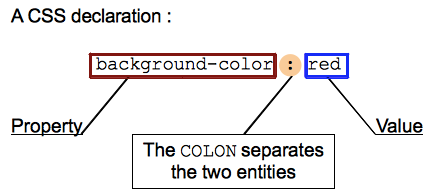
\includegraphics[width=0.9\linewidth]{css_syntax-declaration.png}
\end{center}    

\begin{center}
 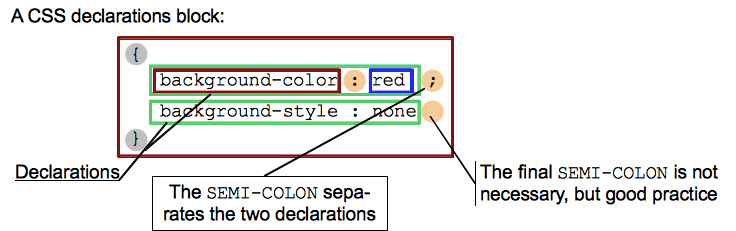
\includegraphics[width=0.9\linewidth]{css_syntax-declarations-block.png}
\end{center}    

\begin{center}
 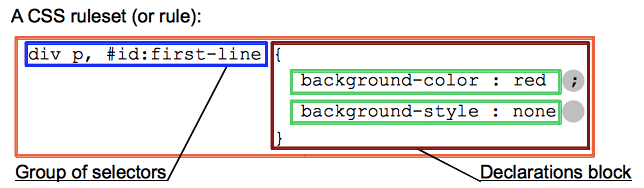
\includegraphics[width=0.9\linewidth]{css_syntax-ruleset.png}
\end{center}    

\begin{codeCSS}{Exemple de syntaxe}
body {
    background-color: white;
    text-align: center;
    color: rgb(15, 15, 15);
}

h1 {
    color: rgb(55, 55, 55);
}
\end{codeCSS}

\subsection{Sélecteurs}
 
\subsection{Liste de propritétés CSS3} 
\begin{itemize}
	\item \url{https://developer.mozilla.org/en-US/docs/Web/CSS/Reference}
\end{itemize}    
    
\end{multicols}
\end{document}